\documentclass{abrice}

\title{Comp 549: Assignment 2}
\author{Anthony Brice}

\begin{document}
\maketitle

\section{Part 1}

\subsection{Sketchpad Demo, Sutherland}

Sutherland's Sketchpad is quite impressive. I had no idea anything remotely like
this existed before GUI operating systems. Their software seems to blur the line
between operating system and program as well. At first they demonstrate some CAD
software, but later they show how to use Sketchpad to write and compile a
flowchart of machine instructions, ``the way a programmer normally operates''
according to the representative.

Sketchpad's 3D modeling technique strikes me as particularly advanced. The TX-2
clearly does not just model lines on a plain, but draws and combines figures of
depth in a three-dimensional space. How anyone managed that with 272KB is
beyond my understanding.

\subsection{Control Devices, Engelbart}

Why does the cable connect to the bottom of the mouse! I suppose I shouldn't be
too critical of a mouse from 1968.

Their chord-based keyboard seems interesting but obviously never took off. I
imagine it's very error prone, and a user would not only have to memorize a
chord for each alphabet character, but also for each special function a typical
keyboard performs. How does one capitalize a letter or delete a character with
the thing?

\subsection{The Three Ways That Good Design Makes You Happy, Norman}

I had no idea the terms breadth-first and depth-first could be applied to human
cognitive processes.

If any design firm has mastered the cues of the visceral, behavioral, and
reflective it's Apple. Their products always look beautiful and striking with
supremely tasteful fonts and construction. They take great care that the user
feels in control of their devices, their touchpads and keyboards have the best
``feel'' of any in their class. Lastly their brand image reflects onto their
users (at least the users hope), providing a sense of erudite sophistication.

\section{Part 2}

\subsection{Man-Computer Symbiosis, Licklider}

I find it funny that Licklider offhandedly almost predicts the Internet with the
line about ``a network of [thinking] centers, connected one another by wide-band
communication lines and to individual users by leased-wire services.'' Like
Vannevar Bush, he doesn't realize that the key to the idea is that the network
be distributed. In his implementation ``users'' make requests to linked ``thinking
centers'' that serve content, but a primary feature of the Internet is that each
node is just as capable of either.

I wonder if he would consider Haskell's and Python's list comprehensions or
Prolog's fact-based consulting as examples of ``computer instruction through
specification of goals.'' Licklider claims that ``Fredkin's trie memory provides
a promising paradigm'' for it, but I fail to see the connection. It seems bizarre
to me to describe such a complex process for something as simple as retrieving a
program for matrix multiplication, but I take the Unix filesystem completely
for granted. It's bizarre even to envision a computer without it.

\subsection{The Computer as a Communication Device, Licklider}

Here we get a more prescient prediction of the Internet as a set of distributed,
networked nodes. The only fault I see is that he's too generous about the
utility of the new network. He envisions that the new network will destroy the
physical barriers barring a user in one location from a program at another, but
fifty years later it's easy to see that the providing a useful networked service
is not quite so simple. From \textsc{CORBA} to \textsc{SOAP} to \textsc{REST},
all kinds of messaging frameworks have come and gone purporting to be the
\textit{right way} to transmit data over the Internet, and the debate is nowhere
near settled.

I like that he immediately recognizes how powerful a tool this new way to
communicate will be, specifically in how it will enable teams to work together
at a previously unimagined level. Surely we can consider the Linux kernel as the
archetypal example of this concept. Thanks to the ability to connect leading
developers across the globe, the kernel has become by far the leading OS kernel
in use, ranging from embedded systems to supercomputers.

I should also note that the essay seems to fall apart at the end. His
description of \textsc{OLIVER} seems to have really nothing to do with ``on-line
communities,'' and is full of the same sort of science fiction fantasies that
precede the introduction of every new personal digital assistant.

\subsection{Human-Centered Computing, Guzdial}

I think Guzdial's thesis that HCI is as much about psychology as it is computing
is sound---the ``Human'' part in the acronym kind of gives it away---but the
overall essay is a little trite. I'd really like to know by what measure ``no
demographic group plays more video games than African-American and Hispanic
teenagers and men'' and if DiSalvo's dissertation really makes that claim. The
impact of her results relies on the claim not in the least.

The claim that ``unlike science or mathematics, undergraduates often come to
computer science with a poor understanding of what computer science is'' is
almost too cute to dissect, but purely anecdotally I know quite a number of math
majors (including my brother who ended up with a PhD. in the field) who went in
as undergraduates thinking they would learn how to do really hard calculus
problems.

\newpage

\section{Part 3}

\begin{figure}
  \centering
  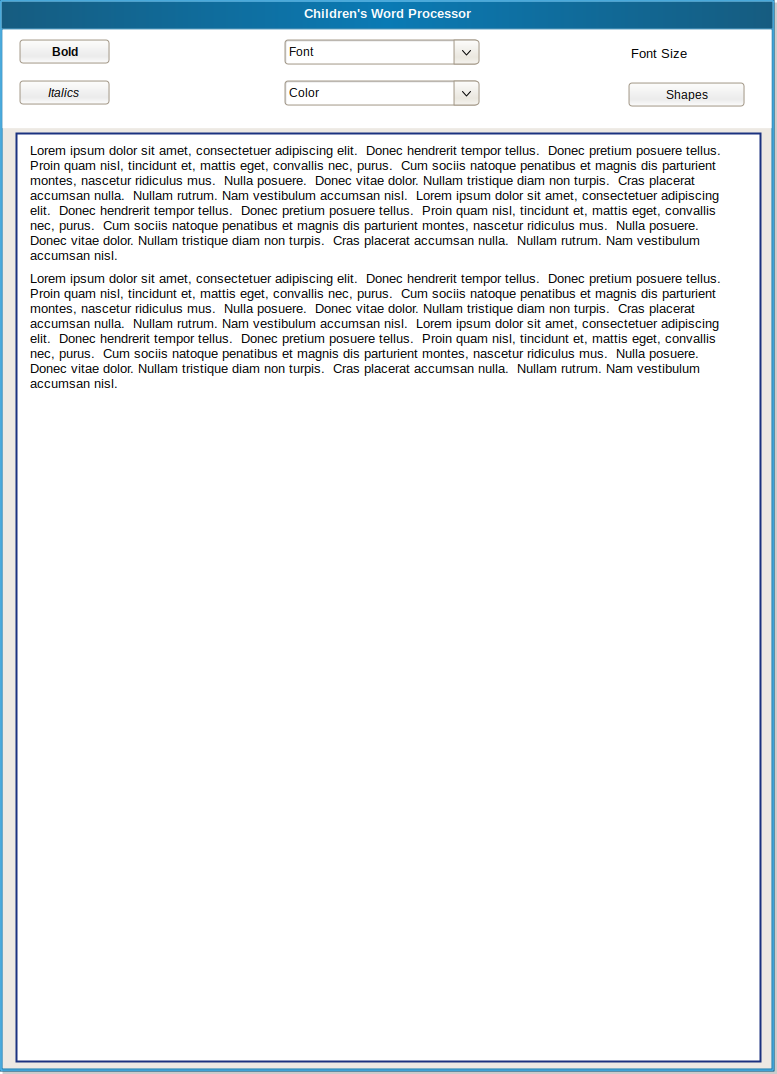
\includegraphics{foobar.png}
  \caption{A GUI for a children's word processor.}
\end{figure}

\begin{figure}
  \centering
  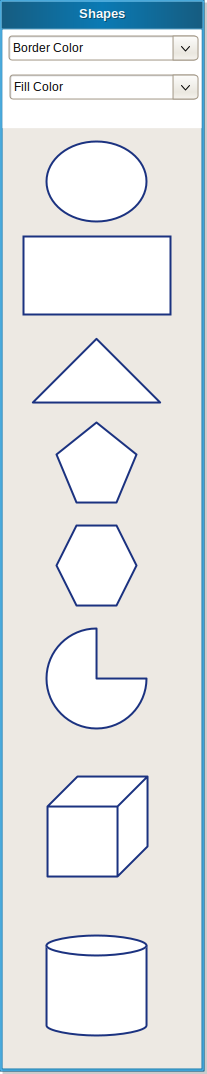
\includegraphics[height=10cm]{shapes.png}
  \caption{The shape selection window.}
\end{figure}

\noindent
I tried to keep my prototype to the bare essentials of word processing so that
children would find it easy to use. The ``Bold,'' ``Italics,'' and ``Shapes''
buttons would clearly indicate their depressed or pressed state. The former two
affect the selected text or text to be typed, and the latter launches the window
shown in Fig.~2. The shapes can be dragged and dropped onto the document with
the pointer.

I specifically chose to forego the advanced functions that many word processors
provide such as templating and list processing because it's so easy to get
trapped in these modes even for a user as old as I am. In my design the state of
any mode should be communicated from the GUI, and a single click will deactivate
said mode.

Shapes can be stacked, resized, and perhaps modified by dragging edges, but I
haven't come up with a good way to allow the user to enter text into an
image. Where does the text get positioned and how can the user modify that
without cluttering and confusing the interface?

\end{document}
%%% Local Variables:
%%% mode: latex
%%% TeX-master: t
%%% End:

%  LocalWords:  Licklider
